%versi 3 (22-07-2020)
\chapter{Landasan Teori}
\label{chap:teori}
Pada bab ini akan menjelaskan dasar teori mengenai Portal Akademik Mahasiswa dan Selenium. 

\section{Portal Akademik Mahasiswa 2018}
\label{sec:pam} 
Portal Akademik Mahasiswa (selanjutnya disingkat dengan PAM) adalah sebuah \textit{web} yang di peruntukan bagi mahasiswa dalam rangka mendapatkan informasi kegiatan akademik mulai dari registrasi, melihat jadwal kuliah dan ujian, info nilai sampai pendaftaran sidang\cite{portalunpar}. Portal Akademik Mahasiswa dapat diakses melalui \url{https://studentportal.unpar.ac.id/}. 

\begin{figure}[H]
	\centering
	
\includegraphics[scale=0.4]{Gambar/halaman2018.jpg}
	\caption{Tampilan halaman awal Portal Akademik Mahasiswa} 
	\label{fig:studpor_home_2018}
\end{figure}

Pada Gambar \ref{fig:studpor_home_2018} adalah tampilan awal ketika masuk ke halaman \url{https://studentportal.unpar.ac.id/}. Mahasiswa perlu melakukan \textit{login} dengan \textit{email} dan \textit{password} mahasiswa UNPAR untuk dapat menggunakan fitur-fitur yang tersedia seperti:
\begin{enumerate}
	\item Fitur mengisi form rencana semester (FRS) atau melakukan perubahan rencana studi (PRS) secara online \\
	Panduan untuk melakukan FRS/PRS online.
	\begin{enumerate}
		\item Masuk ke halaman \url{https://studentportal.unpar.ac.id/} lalu klik tombol ``\textit{Login}'' yang dapat dilihat pada Gambar \ref{fig:studpor_home_2018}
		\item Lakukan ``\textit{Login}'' dengan memasukan email dan password mahasiswa UNPAR pada halaman sso.
		\begin{figure}[H]
			\centering
			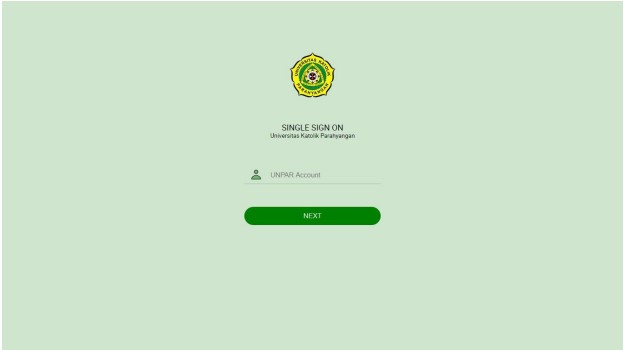
\includegraphics[scale=0.7]{Gambar/sso2018.jpg}
			\caption{Tampilan halaman untuk memasukan \textit{email} Portal Akademik Mahasiswa} 
			\label{fig:sso_2018}
		\end{figure}
	
		\begin{figure}[H]
			\centering
			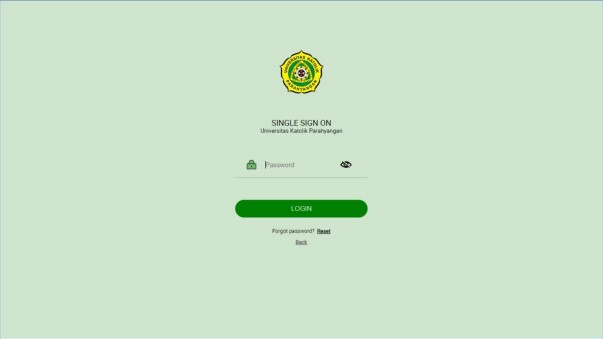
\includegraphics[scale=0.7]{Gambar/pass2018.jpg}
			\caption{Tampilan halaman untuk memasukan \textit{password} Portal Akademik Mahasiswa} 
			\label{fig:pass_2018}
		\end{figure}
		\item Ketika \textit{login} telah berhasil, maka browser akan menampilkan halaman utama, lalu klik pada heksagon berlabel `FRS/PRS' untuk melakukan FRS/PRS online.
		\begin{figure}[H]
			\centering
			
\includegraphics[scale=0.7]{Gambar/frs2018.jpg}
			\caption{Tampilan halaman setelah berhasil \textit{login}} 
			\label{fig:frs_2018}
		\end{figure}
		\item Mahasiswa dapat melakukan FRS sesuai waktu yang sudah ditentukan atau mahasiswa dapat melakukan PRS setelah FRS selesai dan sesuai waktu yang sudah ditentukan untuk PRS.		
	\end{enumerate}
	
	\item Fitur Profil Mahasiswa
	Panduan untuk melihat profil mahasiswa.
	 \begin{enumerate}
	 	\item Mahasiswa melakukan \textit{login} terlebih dahulu. 
	 	\item Menekan menu ``PROFIL'' pada halaman setelah berhasil login seperti pada Gambar \ref{fig:frs_2018}. 
	 	\item Mahasiswa dapat melihat informasi data diri di halaman profil mahasiswa.
	 	\begin{figure}[H]
	 		\centering
	 		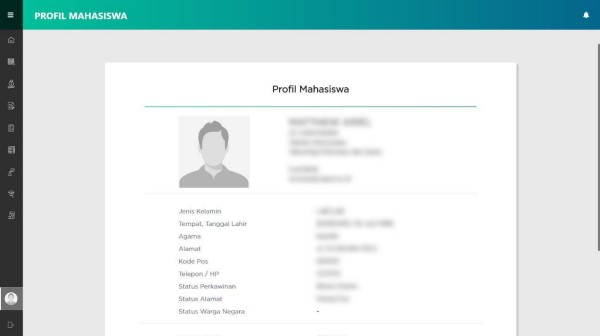
\includegraphics[scale=0.7]{Gambar/profil2018.jpg}
	 		\caption{Tampilan halaman profil mahasiswa} 
	 		\label{fig:profil_2018}
	 	\end{figure}
 	\end{enumerate}
 
	\item Fitur Pembayaran
	Panduan untuk melihat informasi pembayaran.
	\begin{enumerate}
		\item Mahasiswa melakukan \textit{login} terlebih dahulu. 
		\item Menekan menu ``PEMBAYARAN'' pada halaman setelah berhasil login seperti pada Gambar \ref{fig:frs_2018}. 
		\item Pada halaman pembayaran, mahasiswa dapat melihat informasi pembayaran yang terdiri dari Tagihan Pembayaran, Riwayat Pembayaran, dan Keterangan.
	\end{enumerate}
	Pada Gambar \ref{fig:bayar_2018} adalah tabel ``Tagihan Pembayaran'' yang menampilkan jenis tagihan dan jumlah tagihan dari setiap jenis tagihan yang ada.
	\begin{figure}[H]
		\centering
		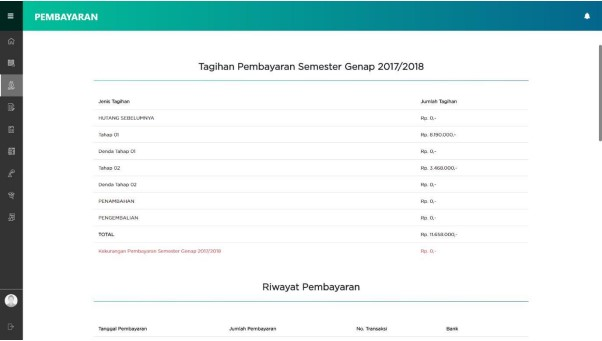
\includegraphics[scale=0.7]{Gambar/bayar2018.jpg}
		\caption{Tampilan halaman pembayaran bagian Tagihan Pembayaran} 
		\label{fig:bayar_2018}
	\end{figure}\\
	
	Pada Gambar \ref{fig:riw_2018} adalah tabel ``Riwayat Pembayaran'' yang menampilkan histori pembayaran yang telah dilakukan.
	\begin{figure}[H]
		\centering
		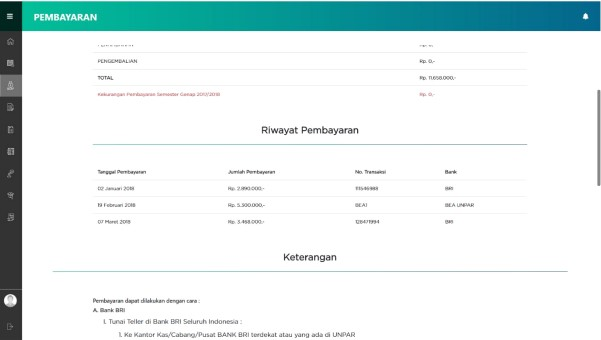
\includegraphics[scale=0.7]{Gambar/riwayat2018.jpg}
		\caption{Tampilan halaman pembayaran bagian Riwayat Pembayaran} 
		\label{fig:riw_2018}
	\end{figure}\\
	
	Pada Gambar \ref{fig:ketbayar_2018} adalah tabel ``Keterangan'' yang menampilkan tata cara pembayaran yang dapat dilakukan untuk melakukan pembayaran.
	\begin{figure}[H]
		\centering
		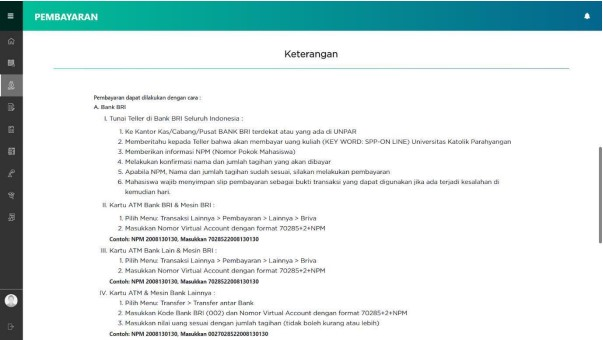
\includegraphics[scale=0.7]{Gambar/keterangan2018.jpg}
		\caption{Tampilan halaman pembayaran bagian Keterangan} 
		\label{fig:ketbayar_2018}
	\end{figure}
	\item Fitur Nilai
	Panduan untuk melihat informasi nilai mahasiswa.
	\begin{enumerate}
		\item Mahasiswa melakukan \textit{login} terlebih dahulu. 
		\item Menekan menu ``NILAI'' pada halaman setelah berhasil login seperti pada Gambar \ref{fig:frs_2018}. 
		\item Pada halaman nilai, mahasiswa dapat melihat informasi nilai dari setiap mata kuliah yang diambil.
		\begin{figure}[H]
			\centering
			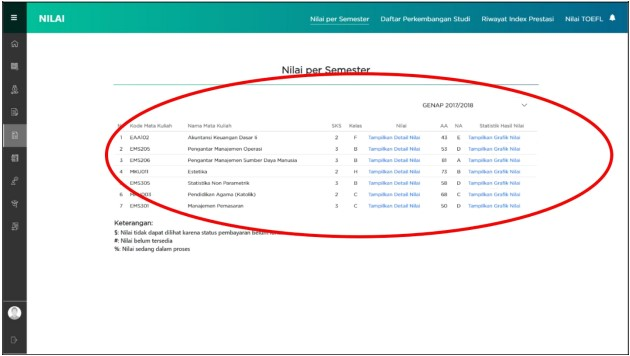
\includegraphics[scale=0.7]{Gambar/nilai2018.jpg}
			\caption{Tampilan halaman nilai bagian Nilai per Semester} 
			\label{fig:nilai_2018}
		\end{figure}
		\item Mahasiswa dapat mengakses menu ``Riwayat Index Prestasi'' untuk melihat `IPK' dan `IPS' mahasiswa.
		\begin{figure}[H]
			\centering
			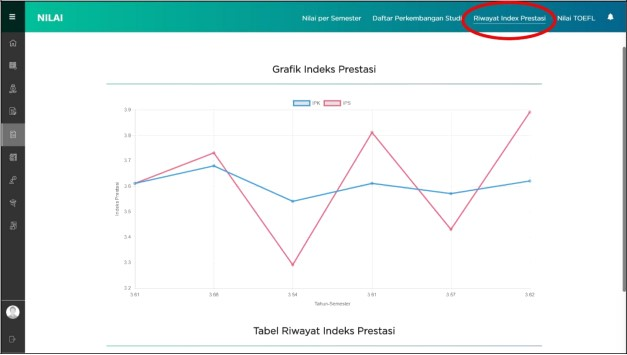
\includegraphics[scale=0.7]{Gambar/rip2018.jpg}
			\caption{Tampilan halaman nilai bagian Riwayat Index Prestasi} 
			\label{fig:rip_2018}
		\end{figure}
	\end{enumerate}	
\end{enumerate}

\section{Selenium}
\label{sec:selenium}
Selenium adalah \textit{open-source} \textit{framework} pengujian otomatisasi untuk aplikasi web\cite{selenium}. Selenium ini adalah WebDriver yang merupakan sebuah \textit{interface} untuk menulis suatu instruksi yang dapat dijalankan secara otomatis dan bergantian pada \textit{browser}.  Selenium WebDriver adalah sebuah \textit{tools} yang berguna untuk melakukan otomatisasi terhadap web pada \textit{browser}. Selenium WebDriver menggunakan API otomatisasi \textit{browser} yang disediakan oleh vendor \textit{browser} untuk mengontrol \textit{browser} dan melakukan pengujian. API WebDriver ini seolah-olah membuat pengguna secara langsung mengoperasi \textit{browser}, padahal dijalankan secara otomatis langsung oleh \textit{API} WebDriver tersebut. Selenium WebDriver ini tersedia untuk bahasa pemrograman Ruby, Java, Python, C\#, dan JavaScript. Selenium WebDriver memiliki berbagai fungsi, yaitu Navigasi \textit{Browser} serta Menemukan elemen.

\subsection{Navigasi \textit{Browser}}
Navigasi \textit{browser} ini berfungsi untuk menjalankan otomatisasi pada browser. Terdapat beberapa metode navigasi \textit{browser}:
\begin{enumerate}
	\item \textit{Navigate to}: hal pertama untuk menggunakan WebDriver adalah melakukan navigasi ke situs web.
	\begin{lstlisting}[language=python, caption=Contoh kode Navigate to, label=kode:2:navigate]
		from selenium import webdriver
		driver = webdriver.Chrome(executable_path='D:\Selenium\chromedriver.exe')
		url = "https://selenium.dev"
		link = driver.get(url)
	\end{lstlisting}
	Pada Kode \ref{kode:2:navigate} merupakan contoh untuk memunculkan situs web yang ingin dijalankan dengan selenium. Baris 1 melakukan \textit{import} webdriver terlebih dahulu, lalu baris 2 \textit{string} dengan nama driver memanggil webdriver yang ingin digunakan, yaitu Google Chrome dan diisi letak file chromedriver.exe disimpan. Baris 3 \textit{string} dengan nama url diisi dengan situs web yang dituju dalam contoh adalah \url{https://selenium.dev}. Baris 4 adalah \textit{string} dengan nama link menggunakan \textit{method get} yang memanggil \textit{string} dengan nama driver yang sudah memanggil webdriver, lalu ditambahkan \textit{method get} yang memanggil \textit{string} dengan nama url yang sudah berisi situs web yang dituju.\\ 
	\item \textit{Get current URL}: untuk membaca URL saat ini dari alamat \textit{browser}.
	\begin{lstlisting}[language=python, caption=Contoh kode Get current URL, label=kode:2:current]
		from selenium import webdriver
		driver = webdriver.Chrome(executable_path='D:\Selenium\chromedriver.exe')
		url = "https://selenium.dev"
		link = driver.get(url)
		current = driver.current_url
		print(current)
	\end{lstlisting}
	Pada Kode \ref{kode:2:current} merupakan contoh untuk membaca situs web yang dijalankan dari \textit{browser}. Pada baris 1 sampai 4 merupakan contoh untuk memunculkan situs web yang ingin dijalankan dengan selenium dan sudah dijelaskan pada Kode \ref{kode:2:navigate}. Baris 5 adalah \textit{string} dengan nama \textit{current} yang memanggil \textit{method current\_url} yang berfungsi untuk mendapatkan situs web dari \textit{browser}. Baris 6 adalah untuk menampilkan situs webnya dengan \textit{method print} dan diisi dengan \textit{string} dengan nama \textit{current} sehingga nantinya akan muncul situs webnya.\\ 
	\item \textit{Back}: menekan tombol kembali pada \textit{browser}.
	\begin{lstlisting}[language=python, caption=Contoh kode Back, label=kode:2:back]
		from selenium import webdriver
		driver = webdriver.Chrome(executable_path='D:\Selenium\chromedriver.exe')
		url = "https://selenium.dev"
		link = driver.get(url)
		kembali = driver.back()
	\end{lstlisting}
	Pada Kode \ref{kode:2:back} merupakan contoh untuk menekan tombol kembali pada \textit{browser}. Pada baris 1 sampai 4 merupakan contoh untuk memunculkan situs web yang ingin dijalankan dengan selenium dan sudah dijelaskan pada Kode \ref{kode:2:navigate}. Baris 5 adalah \textit{string} dengan nama kembali diisi dengan \textit{method back()} yang berfungsi untuk menekan tombol kembali pada \textit{browser}.\\
	\item \textit{Forward}: menekan tombol maju \textit{browser}.
	\begin{lstlisting}[language=python, caption=Contoh kode Forward, label=kode:2:forward]
		from selenium import webdriver
		driver = webdriver.Chrome(executable_path='D:\Selenium\chromedriver.exe')
		url = "https://selenium.dev"
		link = driver.get(url)
		maju = driver.forward()
	\end{lstlisting}
	Pada Kode \ref{kode:2:forward} merupakan contoh untuk menekan tombol maju pada \textit{browser}. Pada baris 1 sampai 4 merupakan contoh untuk memunculkan situs web yang ingin dijalankan dengan selenium dan sudah dijelaskan pada Kode \ref{kode:2:navigate}. Baris 5 adalah \textit{string} dengan nama maju diisi dengan \textit{method forward()} yang berfungsi untuk menekan tombol maju pada \textit{browser}.\\
	\item \textit{Refresh}: melakukan \textit{refresh} halaman.
	\begin{lstlisting}[language=python, caption=Contoh kode Refresh, label=kode:2:refresh]
		from selenium import webdriver
		driver = webdriver.Chrome(executable_path='D:\Selenium\chromedriver.exe')
		url = "https://selenium.dev"
		link = driver.get(url)
		refresh = driver.refresh()
	\end{lstlisting}
	Pada Kode \ref{kode:2:refresh} merupakan contoh untuk menekan tombol \textit{refresh} halaman web pada \textit{browser}. Pada baris 1 sampai 4 merupakan contoh untuk memunculkan situs web yang ingin dijalankan dengan selenium dan sudah dijelaskan pada Kode \ref{kode:2:navigate}. Baris 5 adalah \textit{string} dengan nama \textit{refresh} diisi dengan \textit{method refresh()} yang berfungsi untuk menekan tombol \textit{refresh} halaman web pada \textit{browser}.\\
	\item \textit{Get title}: untuk dapat membaca judul halaman situs web pada \textit{browser}
	\begin{lstlisting}[language=python, caption=Contoh kode Get title, label=kode:2:title]
		from selenium import webdriver
		driver = webdriver.Chrome(executable_path='D:\Selenium\chromedriver.exe')
		url = "https://selenium.dev"
		link = driver.get(url)
		title = driver.title
		print(judul)
	\end{lstlisting}
	Pada Kode \ref{kode:2:title} merupakan contoh untuk membaca judul halaman situs web yang dijalankan dari \textit{browser}. Pada baris 1 sampai 4 merupakan contoh untuk memunculkan situs web yang ingin dijalankan dengan selenium dan sudah dijelaskan pada Kode \ref{kode:2:navigate}. Baris 5 adalah \textit{string} dengan nama \textit{title} yang memanggil \textit{method title} yang berfungsi untuk mendapatkan judul halaman situs web dari \textit{browser}. Baris 6 adalah untuk menampilkan judul situs webnya dengan \textit{method print} dan diisi dengan \textit{string} dengan nama \textit{title} sehingga nantinya akan muncul judul situs webnya.\\ 
	\item \textit{Quit the browser}: untuk dapat keluar dari \textit{browser} setelah selesai menggunakan.
	\begin{lstlisting}[language=python, caption=Contoh kode Get title, label=kode:2:quit]
		from selenium import webdriver
		driver = webdriver.Chrome(executable_path='D:\Selenium\chromedriver.exe')
		url = "https://selenium.dev"
		link = driver.get(url)
		quit = driver.quit()
	\end{lstlisting}
	Pada Kode \ref{kode:2:quit} merupakan contoh untuk dapat keluar dari \textit{browser} setelah selesai menggunakan. Pada baris 1 sampai 4 merupakan contoh untuk memunculkan situs web yang ingin dijalankan dengan selenium dan sudah dijelaskan pada Kode \ref{kode:2:navigate}. Baris 5 adalah \textit{string} dengan nama \textit{quit} yang memanggil \textit{method quit()} yang berfungsi untuk dapat keluar dari \textit{browser} setelah selesai digunakan.
\end{enumerate}

\subsection{Menemukan elemen}
Salah satu teknik mendasar untuk dipelajari saat menggunakan WebDriver adalah cara menemukan elemen di halaman web. WebDriver menyediakan berbagai cara untuk menemukan elemen, terdapat delapan strategi menemukan lokasi elemen yang berbeda di WebDriver:
\begin{enumerate}
	\item Id : Menemukan elemen yang atribut ID-nya cocok dengan nilai pencarian.
	\begin{lstlisting}[language=python, caption=Contoh kode untuk menemukan elemen dengan atribut ID, label=kode:2:elemenid]
		from selenium.webdriver.common.by import By
		driver = webdriver.Chrome(executable_path='D:\Selenium\chromedriver.exe')
		url = "https://selenium.dev"
		driver.find_element(By.ID, "cheese")	
		driver.find_element_by_id("cheese")
	\end{lstlisting}
	Pada Kode \ref{kode:2:elemenid} baris 4 atau 5 merupakan contoh kode yang dapat digunakan untuk menemukan elemen berdasarkan atribut ID dengan nama id ``cheese'' dari situs web \url{https://selenium.dev}. 

	\item \textit{Class name}: Menemukan elemen yang nama kelasnya berisi nilai pencarian.
	\begin{lstlisting}[language=python, caption=Contoh kode untuk menemukan elemen dengan \textit{class name}, label=kode:2:elemenclass]
		from selenium.webdriver.common.by import By
		driver = webdriver.Chrome(executable_path='D:\Selenium\chromedriver.exe')
		url = "https://selenium.dev"
		kelas = driver.find_elements(By.CLASS_NAME, "text-center")
	\end{lstlisting}
	Pada Kode \ref{kode:2:elemenclass} baris 4 merupakan contoh kode untuk mencari elemen dengan \textit{class name} ``text-center'' dan disimpan dalam \textit{string} kelas.
	
	\item \textit{CSS selector}: Menemukan elemen yang cocok dengan pemilihan \textit{Cascading Style Sheets} (CSS). Pemilihan pada CSS adalah pola yang digunakan untuk memilih elemen dengan \textit{style} yang diinginkan .
	\begin{lstlisting}[language=python, caption=Contoh kode untuk menemukan elemen dengan \textit{CSS selector}, label=kode:2:elemencss]
		from selenium.webdriver.common.by import By
		driver = webdriver.Chrome(executable_path='D:\Selenium\chromedriver.exe')
		url = "https://selenium.dev"
		select = driver.find_element(By.CSS_SELECTOR,"#selenium_logo")
	\end{lstlisting}
	Pada Kode \ref{kode:2:elemencss} baris 4 merupakan contoh kode yang disimpan dalam \textit{string} \textit{select} untuk mencari elemen berdasarkan pemilihan CSS dengan mengambil elemen dengan id ``selenium\_logo''.
	
	\item Name: Menemukan elemen yang atribut \textit{name} yang cocok dengan nilai pencarian. 
	\begin{lstlisting}[language=python, caption=Contoh kode untuk menemukan elemen dengan atribut nama, label=kode:2:elemenname]
		from selenium.webdriver.common.by import By
		driver = webdriver.Chrome(executable_path='D:\Selenium\chromedriver.exe')
		url = "https://www.facebook.com/"
		nama = driver.find_element(By.NAME,"email")
	\end{lstlisting}
	Pada Kode \ref{kode:2:elemenname} baris 4 mencari elemen dari atribut namanya dari situs web \url{https://www.facebook.com/} dengan atribut namanya adalah ``email'' dan disimpan dalam \textit{string} nama.
	
	\item link text: Menemukan elemen \textit{link} yang teksnya terlihat cocok dengan nilai pencarian.
	\begin{lstlisting}[language=python, caption=Contoh kode untuk menemukan elemen dengan \textit{link text}, label=kode:2:elemenlink]
		from selenium.webdriver.common.by import By
		driver = webdriver.Chrome(executable_path='D:\Selenium\chromedriver.exe')
		url = "https://selenium.dev"
		nama = driver.find_element(By.LINK_TEXT, "Documentation")
	\end{lstlisting}
	Pada Kode \ref{kode:2:elemenlink} baris 4 mencari elemen \textit{link} yang dengan nama teksnya adalah ``Documentation'' dari situs web \url{https://selenium.dev}
	
	\item partial link text: Menemukan elemen \textit{link} yang teksnya terlihat berisi nilai pencarian. Jika beberapa elemen cocok, hanya yang pertama yang akan dipilih.
	\begin{lstlisting}[language=python, caption=Contoh kode untuk menemukan elemen dengan \textit{partial link text}, label=kode:2:elemenpartial]
		from selenium.webdriver.common.by import By
		driver = webdriver.Chrome(executable_path='D:\Selenium\chromedriver.exe')
		url = "https://selenium.dev"
		nama = driver.find_element(By.PARTIAL_LINK_TEXT, "About Selenium")
	\end{lstlisting}
	Pada Kode \ref{kode:2:elemenpartial} baris 4 mencari elemen \textit{link} yang dengan nama teksnya adalah ``About Selenium'' dari situs web \url{https://selenium.dev}, namun ketika ada beberapa elemen yang cocok dengan nama teks yang dicari maka akan diambil yang pertamanya saja.
	
	\item tag name: Menemukan elemen yang nama tagnya cocok dengan nilai pencarian.
	\begin{lstlisting}[language=python, caption=Contoh kode untuk menemukan elemen dengan \textit{tag name}, label=kode:2:elementag]
		from selenium.webdriver.common.by import By
		driver = webdriver.Chrome(executable_path='D:\Selenium\chromedriver.exe')
		url = "https://selenium.dev"
		tag = driver.find_element(By.TAG_NAME, "h1")
	\end{lstlisting}
	Pada Kode \ref{kode:2:elementag} baris 4 mencari elemen yang nama tagnya adalah ``h1'' dari situs web \url{https://selenium.dev} yang disimpan dengan \textit{string} \textit{tag}.
	
	\item XPath: Menemukan elemen yang cocok dengan ekspresi \textit{XML Path Language} (XPath).
	\begin{lstlisting}[language=python, caption=Contoh kode untuk menemukan elemen dengan ekspresi XPath, label=kode:2:elemenxpath]
		from selenium.webdriver.common.by import By
		driver = webdriver.Chrome(executable_path='D:\Selenium\chromedriver.exe')
		url = "https://selenium.dev"
		contoh1 = driver.find_element(By.XPATH, "//*[@id='td-cover-block-0']/div/div/div/div/h1")
		contoh2 = driver.find_element(By.XPATH, "/html/body/div/main/section[1]/div/div/div/div/h1")
	\end{lstlisting}
	Pada Kode \ref{kode:2:elemenxpath} baris 4 mencari elemen dengan XPath mulai dari nama id dari element yang dicari adalah `td-cover-block-0', lalu diarahkan hingga tempat elemen yang dicari itu berada, dan disimpan di \textit{string} contoh1. Pada baris 5 mencari elemen dengan XPath yang mulai dari struktur webnya dari atas hingga menuju tempat elemen itu berada dan disimpen di \textit{string} contoh2.

\end{enumerate}


\subsection{Waits}
WebDriver secara umum dapat dikatakan memiliki API pemblokiran. Karena ini adalah \textit{library} di luar proses yang menginstruksikan browser apa yang harus dilakukan, dan karena platform web secara intrinsik memiliki sifat asinkron, WebDriver tidak melacak status document object model (DOM) yang aktif dan real-time. Selenium WebDriver memiliki tiga tipe waits:
\begin{enumerate}
	\item Implicit wait: memberi tahu WebDriver untuk melakukan polling DOM selama jangka waktu tertentu ketika mencoba menemukan elemen atau elemen jika tidak segera tersedia. Pengaturan default adalah 0, artinya dinonaktifkan. Setelah disetel, penantian implisit disetel untuk masa pakai sesi.
	\begin{lstlisting}[language=python, caption=Contoh kode Implicit wait, label=kode:2:implicit]
		driver = Firefox()
		driver.implicitly_wait(10)
		driver.get("http://somedomain/url_that_delays_loading")
		my_dynamic_element = driver.find_element(By.ID, "myDynamicElement")
	\end{lstlisting}
	\item Explicit wait: mengizinkan kode untuk menghentikan eksekusi program, atau membekukan \textit{thread}, hingga suatu kondisi dapat teratasi. Kondisi ini dipanggil dengan frekuensi tertentu sampai batas waktu tunggu terlewati.
	\begin{lstlisting}[language=python, caption=Contoh kode Explicit wait, label=kode:2:explicit]
		from selenium.webdriver.support.ui import WebDriverWait
		
		driver.navigate("file:///race_condition.html")
		el = WebDriverWait(driver).until(lambda d: d.find_element_by_tag_name("p"))
		assert el.text == "Hello from JavaScript!"
	\end{lstlisting}
	\item Fluent wait: menentukan jumlah waktu maksimum untuk menunggu suatu kondisi, serta frekuensi untuk memeriksa kondisi tersebut.
	\begin{lstlisting}[language=python, caption=Contoh kode FluentWait, label=kode:2:FluentWait]
		driver = Firefox()
		driver.get("http://somedomain/url_that_delays_loading")
		wait = WebDriverWait(driver, 10, poll_frequency=1, ignored_exceptions=[ElementNotVisibleException, ElementNotSelectableException])
		element = wait.until(EC.element_to_be_clickable((By.XPATH, "//div")))
	\end{lstlisting}
\end{enumerate}










